\section{The Radon transform}
The \textit{Radon transform} defines projections of an object mapping it from its spatial domain to its projection space. That is, using the Radon transform on a 2D object from a single angle, we obtain a 1D projection of the object which can be interpreted as a histogram of the objects density from that angle. Having a 2D object, $f(x,y)$, defined in the spatial domain and the rectangular coordinate system, the Radon transform is defined as the projection $(p,\theta)$ in the polar coordinate system:
\begin{equation} \label{linearity}
	P(p,\theta) = \mathbf{R}\{f(x,y)\} = \int_L f(x,y) dl
\end{equation}  
Where $\int_L$ is the line integral defined along the path \textit{L}, such that $xcos(\theta) + ysin(\theta) = p$. The polar coordinate system, $(p,\theta)$, can be translated into rectangular coordinates by using a rotated coordinate system $(p,q)$ where:
\begin{align*}
	xcos(\theta) + ysin(\theta) &= p \\
	-xsin(\theta) + ycos(\theta) & = q
\end{align*}
This change of coordinates implies an equivalent definition of the Radon transform in terms of polar coordinates:
\begin{equation*}
	\mathbf{R}\{f(x,y)\} = \int_{-\infty}^{\infty}f(pcos(\theta) - qsin(\theta),psin(\theta)+qcos(\theta))dq
\end{equation*}
For a fixed angle $\theta$ the 1D function $P_{\theta}(p) = P(p,\theta)$ and is called a projection. It contains all line integrals over $f(x,y)$ with the constant angle $\theta$ and variable distance $p$ to the origin, and as described earlier, can be interpreted as a histogram of the objects density from this angle.\\
\begin{figure}
	\centering
	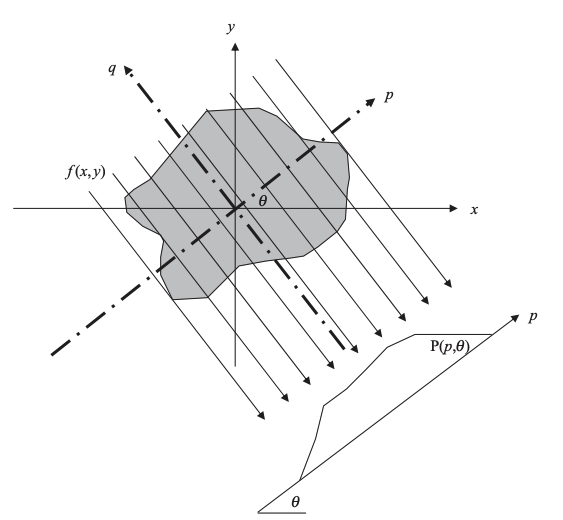
\includegraphics[width=\linewidth]{Materials/Projection}
	\caption{2D object $f(x,y)$ shown as shaded object in the rectangular coordinate system $(x,y)$. The lines indicate the direction the line integrals are computed, and are defined by the angle $\theta$ and sampled along the $p$ axis from the rotated coordinate system $(p,q)$. As a result of computing the line integrals, we see the 1D projection $P(p,\theta)$ in the bottom of the image. Image is from \cite{MIA}.}
	\label{projection}
\end{figure}
In \autoref{projection} we see a projection of a 2D object. We see the shaded object defined in the rectangular coordinate system $(x,y)$ and the lines for which the line integrals are taken along. The lines are defined by the angle $\theta$, and by taking the line integrals from $-\infty$ to $\infty$ we get the projection seen in the lower right of the image. We see how a 'high response' is measured when the object is wide along the lines, and a 'low response' when the object is narrow.\\
If we take the Radon transform over several angles we can concatenate the produced projections and construct a \textit{sinogram}. A sinogram has the angles sampled along the $x-axis$ and the distances $p$ along the $y-axis$. In \autoref{sino} we see a sinogram computed over a uniform circle. As the circle is not centered at the origin, the sinogram gets a curved shape because as we rotate around the circle the relative position to the projection plane shifts.

\begin{figure}
	\centering
	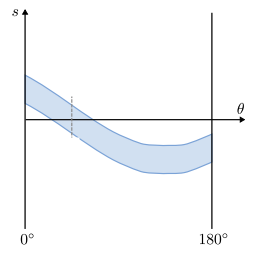
\includegraphics[width=0.5\linewidth]{Materials/sino}
	\caption{A sinogram computed over a uniform circle. Image from \cite{MIA}.}
	\label{sino}
\end{figure}